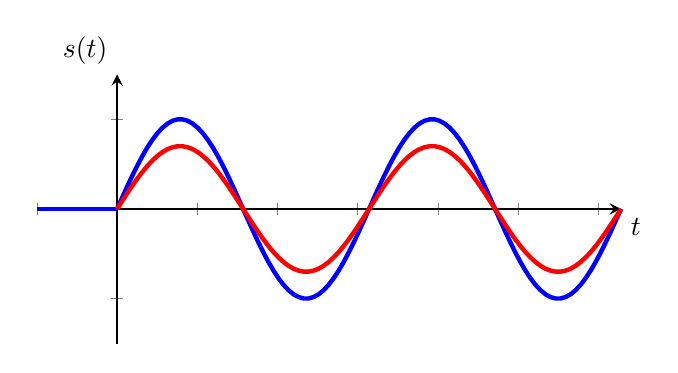
\begin{tikzpicture}
\begin{axis}[
        axis line style = thick,
        clip=false,
        height=5cm,
        width=9cm,
        axis x line=center,
        axis y line=center,
        xmin=-2,
        xmax=4*pi,
        ymin=-1.5,
        ymax=1.5,
        xlabel={$t$},
        ylabel={$s(t)$},
        xlabel style={below right},
        ylabel style={above left},
        ytick={-1,1},
        yticklabels={},
        xtick={},
        xticklabels={},
        ]

            \addplot [ultra thick,color=blue,domain=-2:0, samples=101]{0};
            \addplot [ultra thick,color=blue,domain=0:4*pi, samples=101]{sin(deg(x))};
            \addplot [ultra thick,color=red,domain=0:4*pi, samples=101]{0.7*sin(deg(x))};
        \end{axis}
\end{tikzpicture}
